% $Id: template.tex 11 2007-04-03 22:25:53Z jpeltier $

\documentclass{vgtc}                          % final (conference style)
%\documentclass[review]{vgtc}                 % review
%\documentclass[widereview]{vgtc}             % wide-spaced review
%\documentclass[preprint]{vgtc}               % preprint
%\documentclass[electronic]{vgtc}             % electronic version

%% Uncomment one of the lines above depending on where your paper is
%% in the conference process. ``review'' and ``widereview'' are for review
%% submission, ``preprint'' is for pre-publication, and the final version
%% doesn't use a specific qualifier. Further, ``electronic'' includes
%% hyperreferences for more convenient online viewing.

%% Please use one of the ``review'' options in combination with the
%% assigned online id (see below) ONLY if your paper uses a double blind
%% review process. Some conferences, like IEEE Vis and InfoVis, have NOT
%% in the past.

%% Figures should be in CMYK or Grey scale format, otherwise, colour 
%% shifting may occur during the printing process.

%% These few lines make a distinction between latex and pdflatex calls and they
%% bring in essential packages for graphics and font handling.
%% Note that due to the \DeclareGraphicsExtensions{} call it is no longer necessary
%% to provide the the path and extension of a graphics file:
%% \includegraphics{diamondrule} is completely sufficient.
%%
\ifpdf%                                % if we use pdflatex
  \pdfoutput=1\relax                   % create PDFs from pdfLaTeX
  \pdfcompresslevel=9                  % PDF Compression
  \pdfoptionpdfminorversion=7          % create PDF 1.7
  \ExecuteOptions{pdftex}
  \usepackage{graphicx}                % allow us to embed graphics files
  \DeclareGraphicsExtensions{.pdf,.png,.jpg,.jpeg} % for pdflatex we expect .pdf, .png, or .jpg files
\else%                                 % else we use pure latex
  \ExecuteOptions{dvips}
  \usepackage{graphicx}                % allow us to embed graphics files
  \DeclareGraphicsExtensions{.eps}     % for pure latex we expect eps files
\fi%

%% it is recomended to use ``\autoref{sec:bla}'' instead of ``Fig.~\ref{sec:bla}''
\graphicspath{{figures/}{pictures/}{images/}{./}} % where to search for the images

\usepackage{microtype}                 % use micro-typography (slightly more compact, better to read)
\PassOptionsToPackage{warn}{textcomp}  % to address font issues with \textrightarrow
\usepackage{textcomp}                  % use better special symbols
\usepackage{mathptmx}                  % use matching math font
\usepackage{times}                     % we use Times as the main font
\renewcommand*\ttdefault{txtt}         % a nicer typewriter font
\usepackage{cite}                      % needed to automatically sort the references
\usepackage{tabu}                      % only used for the table example
\usepackage{booktabs}                  % only used for the table example
%% We encourage the use of mathptmx for consistent usage of times font
%% throughout the proceedings. However, if you encounter conflicts
%% with other math-related packages, you may want to disable it.


%% If you are submitting a paper to a conference for review with a double
%% blind reviewing process, please replace the value ``0'' below with your
%% OnlineID. Otherwise, you may safely leave it at ``0''.
\onlineid{0}

%% declare the category of your paper, only shown in review mode
\vgtccategory{Research}

%% allow for this line if you want the electronic option to work properly
\vgtcinsertpkg

%% In preprint mode you may define your own headline.
%\preprinttext{To appear in an IEEE VGTC sponsored conference.}

%% Paper title.

\title{Global Illumination for Fun and Profit}

%% This is how authors are specified in the conference style

%% Author and Affiliation (single author).
%%\author{Roy G. Biv\thanks{e-mail: roy.g.biv@aol.com}}
%%\affiliation{\scriptsize Allied Widgets Research}

%% Author and Affiliation (multiple authors with single affiliations).
%%\author{Roy G. Biv\thanks{e-mail: roy.g.biv@aol.com} %
%%\and Ed Grimley\thanks{e-mail:ed.grimley@aol.com} %
%%\and Martha Stewart\thanks{e-mail:martha.stewart@marthastewart.com}}
%%\affiliation{\scriptsize Martha Stewart Enterprises \\ Microsoft Research}

%% Author and Affiliation (multiple authors with multiple affiliations)
\author{Alberto Chan Liu\thanks{e-mail: albertochanliu2018@gmail.com}\\ %
         %
\and Irene Zhang\thanks{e-mail: irenezhang342@gmail.com}\\ %
      %
\and Zhipeng Yang\thanks{e-mail: yangzhipeng666@gmail.com}\\ %
     }

%% A teaser figure can be included as follows, but is not recommended since
%% the space is now taken up by a full width abstract.
\teaser{
  \centering
 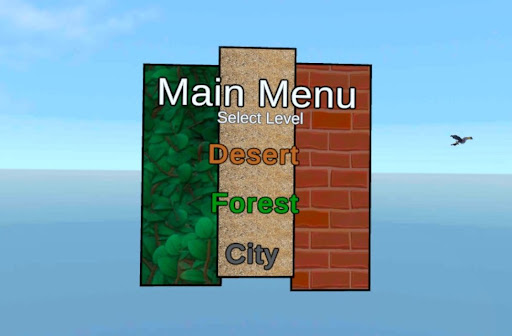
\includegraphics[width=5in]{menu.jpg}
 \caption{Main Menu}
}

%% Abstract section.
\abstract{This project will provide a playable environment using a VR 
set, specifically the Oculus Quest 2, in which the user will be able 
to interact with a virtual world as a character and enjoy the different 
challenges the environment will provide to them. The challenges will 
consist of a set of obstacles different to each other and specific to 
the different environments. The user will have to pass through all 
obstacles by jumping, running or moving in order to get to the end 
of each of the virtual worlds and win each level environment before 
the time ends..%
} % end of abstract

%% ACM Computing Classification System (CCS). 
%% See <http://www.acm.org/about/class> for details.
%% We recommend the 2012 system <http://www.acm.org/about/class/class/2012>
%% For the 2012 system use the ``\CCScatTwelve'' which command takes four arguments.
%% The 1998 system <http://www.acm.org/about/class/class/2012> is still possible
%% For the 1998 system use the ``\CCScat'' which command takes four arguments.
%% In both cases the last two arguments (1998) or last three (2012) can be empty.

\CCScatlist{
  \CCScatTwelve{Virtual reality}{Game design}{Obstacle course}{Interaction};
}

%\CCScatlist{
  %\CCScat{H.5.2}{User Interfaces}{User Interfaces}{Graphical user interfaces (GUI)}{};
  %\CCScat{H.5.m}{Information Interfaces and Presentation}{Miscellaneous}{}{}
%}

%% Copyright space is enabled by default as required by guidelines.
%% It is disabled by the 'review' option or via the following command:
% \nocopyrightspace

%%%%%%%%%%%%%%%%%%%%%%%%%%%%%%%%%%%%%%%%%%%%%%%%%%%%%%%%%%%%%%%%
%%%%%%%%%%%%%%%%%%%%%% START OF THE PAPER %%%%%%%%%%%%%%%%%%%%%%
%%%%%%%%%%%%%%%%%%%%%%%%%%%%%%%%%%%%%%%%%%%%%%%%%%%%%%%%%%%%%%%%%

\begin{document}

%% The ``\maketitle'' command must be the first command after the
%% ``\begin{document}'' command. It prepares and prints the title block.

%% the only exception to this rule is the \firstsection command
\firstsection{Introduction}

\maketitle
This game idea is the result of a common interest in our group of understanding the enjoyment from interaction of the user in a game using VR and the different methods used to achieve this goal. All members of the group have tried gaming with technology and found ourselves interested in applying VR to create our own interactive environment and challenge ourselves to create an enjoyable game for the user. 			
\\
Our objective is to use Unity to create three different scenes in which a character controlled by the user will have to get to the end of the map avoiding different obstacles along the way by jumping and running away from the objects created to stop the character. 
\\
The game will provide an enjoyable environment for the user to get distracted from the stress of the real world and find interactive challenges that will be fun to overcome while using the Oculus Quest 2 headset. Our goal is to produce a running VR obstacle game containing three levels, forest, desert, and city. This game is intentionally designed to have increasing levels of difficulty as levels progress. The overall goal is to have people playing this game engage in the fun challenging levels we designed and also have a great time.
 



\section{Related Wrok}
Previous researches like {E}valuating {E}njoyment, {P}resence, and {E}mulator {S}ickness in VR games based on first- and third- person {V}iewing {P}erspectives. In this research, Monteiro \emph{et.~al.}\cite{monteiro_liang_xu_brucker_nanjappan_yue_2018} found out that when using VR headset in a virtual environment game based on a first-person perspective can lead to simulator sickness and discomfort from the user. Whereas in a third person perspective it is less likely that simulator sickness occurs. However in a third person display, the immersiveness of the game is lost.

Our group was put in the dilemma of doing a third person perspective or a first person perspective. We wanted to make an enjoyable game for all users and not worry about motion sickness, but the virtual reality aspect and immersiveness that we were looking for for the project was not going to be there. Since our project is still in development we are still in discussion on what would be the best solution for this problem.

We implemented some environment interactions and objects and Unity techniques to build and run our scenes on Android platform from different online tutorials.~\cite{youtube_2020}

\begin{figure}[tb]
  \centering % avoid the use of \begin{center}...\end{center} and use \centering instead (more compact)
  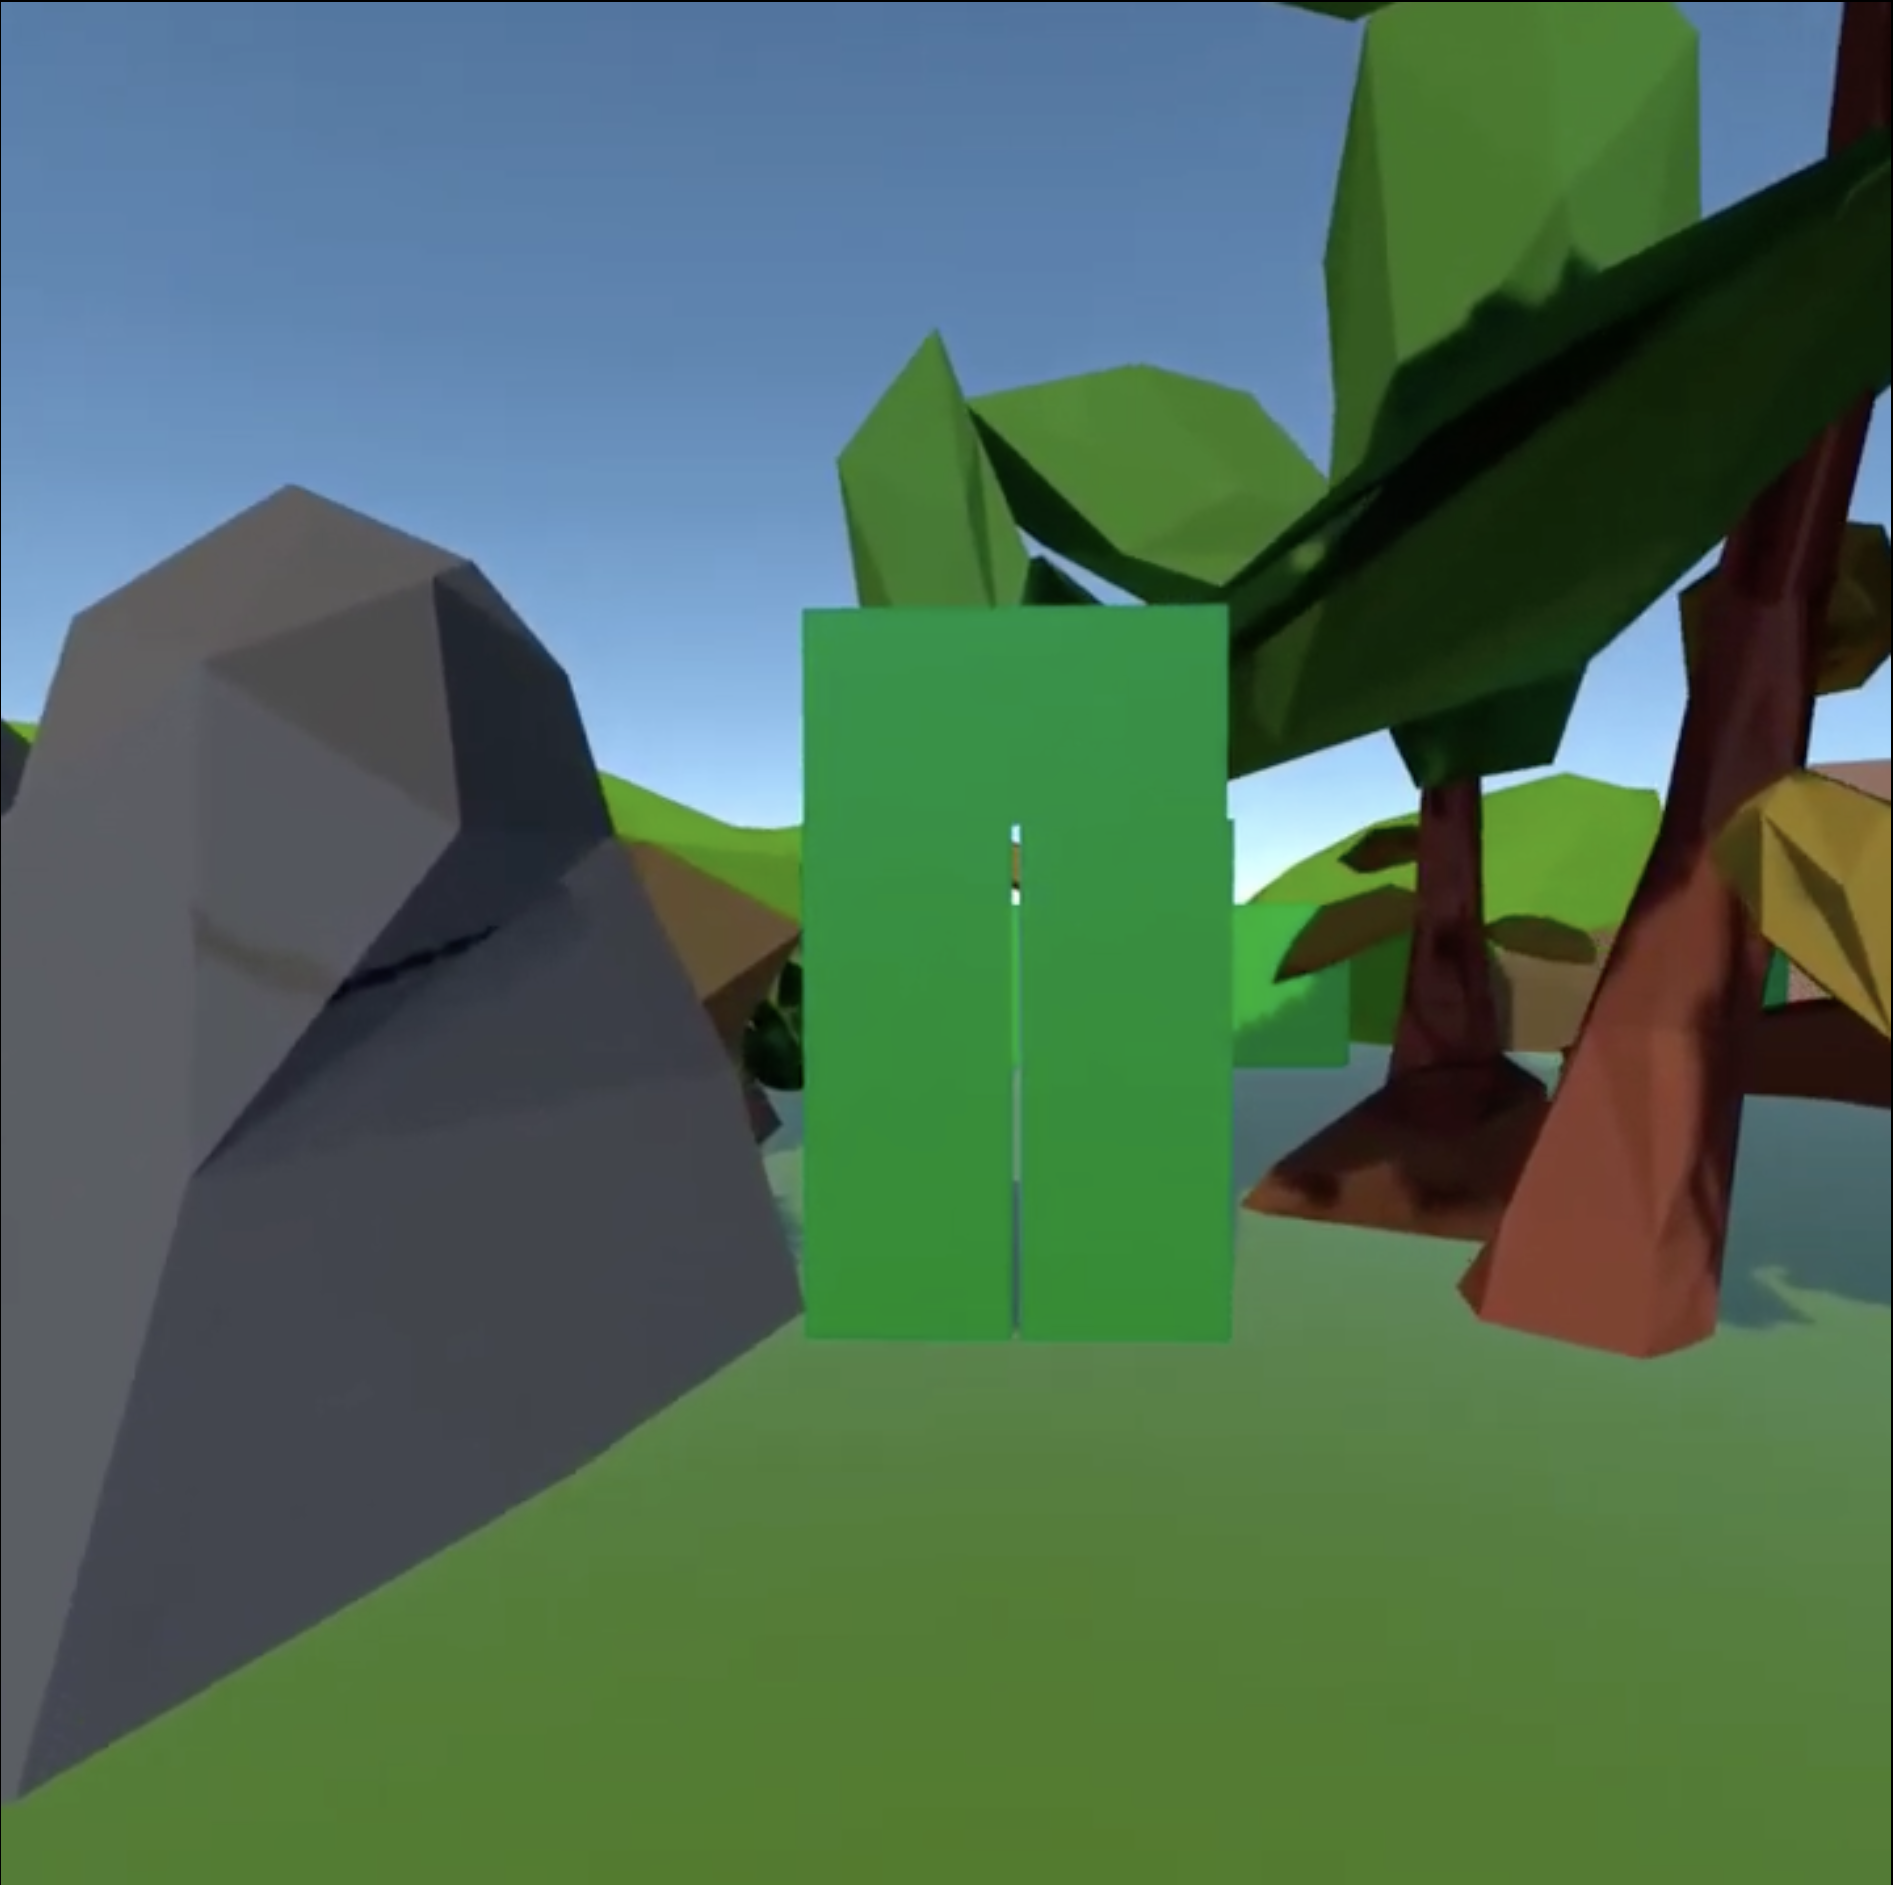
\includegraphics[width=\columnwidth]{forest.png}
  \caption{A visualization of the forest scene}
 \end{figure}

\section{Methods}
This project started as a basic obstacle course game from an Unity Asset Store package called “Obstacle Course Pack” (AisuKase Studio, 2018). This package contained different elements and a movable player that could jump and move with keyboard controls.

To implement this package and the obstacle concept of the game into Virtual Reality, we had to create our own 3D world and make the Quest 2 headset work with Unity, which caused some problems since our team members had Apple devices and Unity needed to be configured manually to work with macOS systems. After overcoming our own obstacles we proceed to create the different level scenarios, specifically Desert, Forest and City and using different assets from various resources online, we could create an environment that simulated the desired world setting.
\begin{figure}[tb]
  \centering % avoid the use of \begin{center}...\end{center} and use \centering instead (more compact)
  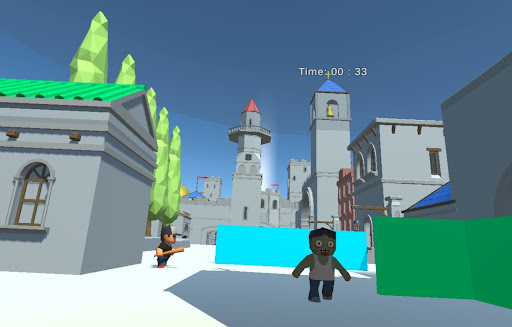
\includegraphics[width=\columnwidth]{city1.jpg}
  \caption{A visualization of the city scene}
 \end{figure}

 \begin{figure}[tb]
  \centering % avoid the use of \begin{center}...\end{center} and use \centering instead (more compact)
  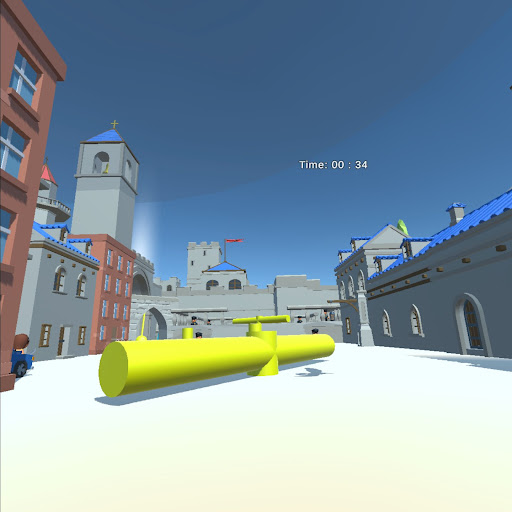
\includegraphics[width=\columnwidth]{city2.jpg}
  \caption{A visualization of the city scene}
 \end{figure}
To make the game more challenging and make the objective of the game not solely to get to the end, we implemented a timer that was attached to the headset view.  With this timer the user will have to be focused on going through all the obstacles and get to the end of the level as fast as possible before the time ends and the screen displays a game over scene or try again.

The game will be playable with a Quest 2 VR headset and control joystick will be used to move and turn the character.  Control main triggers will be used to make the character jump. We had to ensure that the user played in a safe environment since the user will be immersed in a virtual world and will not have visual contact with the real world. To do that we limited the movement from our controls to interact as little as possible.  

On the Desert level, interaction with the environment included grabbing rocks with the secondary triggers. The rocks were interactable to be used to throw them at animated chickens (chickens are subject to change due to animal rights) and when the rock made contact with the chicken the user would get more time added to finish the level.

There are some interactions used in desert city scene. Users are able to control their moving direction by VR headset. Players can control their jump by the main trigger of the touch controller. In addition, we have a countdown timer. When the player collides with obstacles, players will be pushed back or bounced into the sky, and it will waste players’ time.When players run out of time, the game will show a game  over menu, and players can choose “try again” or “quit game”. When players reach the finish line, there is an event trigger which will take players to the congratulations menu,and they can choose the next level scene. 

Throughout the design phase of our VR game, many interaction methods were employed to create a fuller player experience. For interactions, the end goal of our project is to have players complete obstacle challenges in virtual reality through some minimal physical movements. For reference frames, the forest level is intended to use the torso reference frame which moves with both physical and virtual rotation. In terms of user locomotion, we plan to have users stay in place while also having control to character movement through the controller. We aim to minimize user moving range but add as many in-place movements as possible for safety considerations. We decided to use controllers over bare hands because of their features of reliability and capability of adding haptics.
\begin{figure}[tb]
  \centering % avoid the use of \begin{center}...\end{center} and use \centering instead (more compact)
  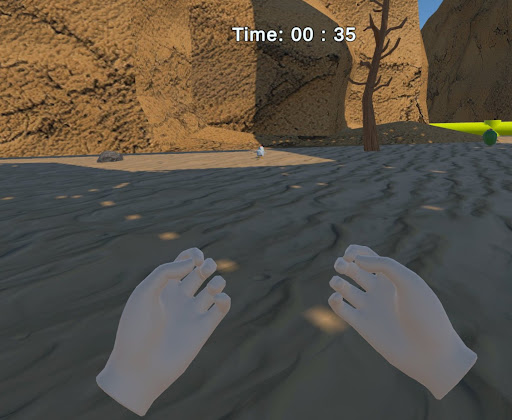
\includegraphics[width=\columnwidth]{desert1.jpg}
  \caption{A visualization of the desert scene}
 \end{figure}
\begin{figure}[tb]
  \centering % avoid the use of \begin{center}...\end{center} and use \centering instead (more compact)
  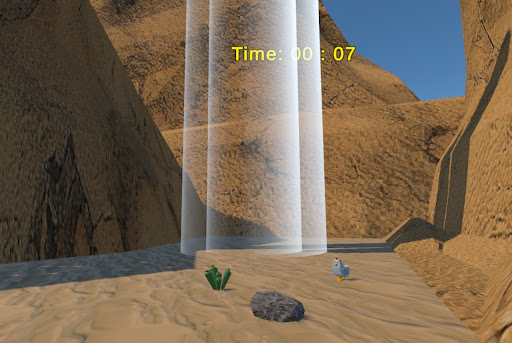
\includegraphics[width=\columnwidth]{desert2.jpg}
  \caption{A visualization of the desert scene}
 \end{figure}
\section{User Evaluation and Results}
The obstacle game starts with the main menu which includes buttons of the three main levels and three eagles flying around with sound effects and game music that made the user of the game feel comfortable and prepared them to start the game. Once it chooses the level desired to play, the user is immediately put into the start of the level chosen to play and timer starts running, this makes the user of the game  change its focus immediately to look at the world created by us and start looking for a way to reach the end point of the level.

We notice that users that are not familiar with the usage of VR systems will tend to feel motion sickness when the game is played for a long time so we decided to make the timer be less than 2 minutes and be able to be personalized in Unity.

As an added interaction with the obstacles we made the player bounce against some of the movable obstacles and in some levels play a sound that seemed enjoyable by the users. Although not all the interactions with objects work efficiently and as desired, like the feeling of going through objects and some objects pushing the user too far, the game still was enjoyable.

At the end menus of the game we added a scene for winning the game and losing. In both of these scenes we included an animated chicken so that the player could also visually enjoy the end of the game even if the outcome was not as desired.

\begin{figure}[tb]
  \centering % avoid the use of \begin{center}...\end{center} and use \centering instead (more compact)
  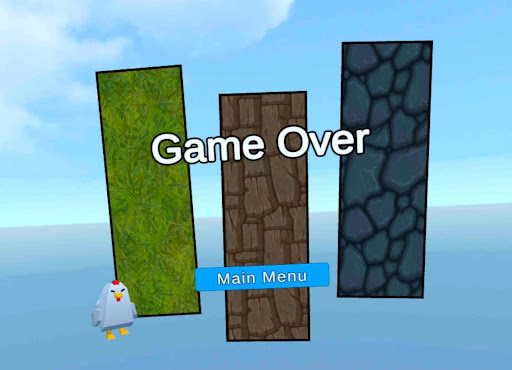
\includegraphics[width=\columnwidth]{end menu.jpg}
  \caption{Game Over}
 \end{figure}
\section{Discussions and Conclusions}
Using Unity and all its features to create our virtual reality worlds was really challenging and beneficial to us since it  put our programming skills and creativity to work. Unity is a really powerful tool for developers like us to be creative and use this program to make more than just games, but real intricate applications compatible with Virtual Reality, Augmented Reality, Mixed Reality and much more.

The decision to change the main character from a third person player to a first person player was the best idea for our project to be more immersive and interactable for the user. It made the controls and movement more natural for a person and the interactions more real.

Our obstacle game resulted in a really enjoyable VR game that challenged the user to interact with different objects and obstacles included on the levels created by us. The user  by going through our personalized immersive worlds and drawing players into a reality made by us.

\begin{figure}[tb]
  \centering % avoid the use of \begin{center}...\end{center} and use \centering instead (more compact)
  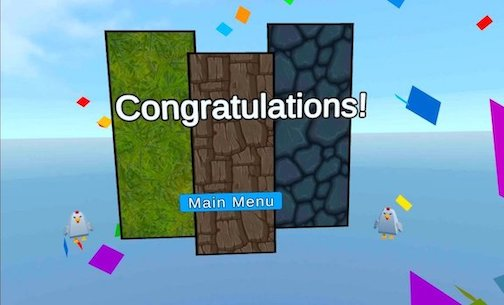
\includegraphics[width=\columnwidth]{cong.jpeg}
  \caption{Congratulations}
 \end{figure}
%% if specified like this the section will be committed in review mode
% \acknowledgments{
% The authors wish to thank A, B, and C. This work was supported in part by
% a grant from XYZ.}

%\bibliographystyle{abbrv}
\bibliographystyle{abbrv-doi}
%\bibliographystyle{abbrv-doi-narrow}
%\bibliographystyle{abbrv-doi-hyperref}
%\bibliographystyle{abbrv-doi-hyperref-narrow}

\bibliography{VR_Final_Report}
\end{document}
